\documentclass[aspectratio=169, 10pt]{beamer}

\usepackage{bm} % bold math
\usepackage{fontspec}
\usepackage{minted}
\usepackage{pgf-pie}
\usepackage{tikz}

% Custom commands and environments
\makeatletter
\newcommand\version[1]{\renewcommand\@version{#1}}
\newcommand\@version{}
\def\insertversion{\@version}

\newcommand\course[1]{\renewcommand\@course{#1}}
\newcommand\@course{}
\def\insertcourse{\@course}

\newcommand\coursetitle[1]{\renewcommand\@coursetitle{#1}}
\newcommand\@coursetitle{}
\def\insertcoursetitle{\@coursetitle}

\newcommand\lecturenumber[1]{\renewcommand\@lecturenumber{#1}}
\newcommand\@lecturenumber{}
\def\insertlecturenumber{\@lecturenumber}
\makeatother

\newcommand{\slidetitle}[1]{{\xbseries \large \structure{#1}} \bigskip}
\newcommand{\term}[1]{{\color{blue} #1}}
\newcommand{\leftspace}{\hspace{1em}}
\newcommand{\inlinearrow}{
  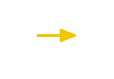
\begin{tikzpicture}[baseline]
    \node [anchor=base] (x) {};
    \draw [rawarrow] (x.mid west) -- ($(x.mid west) + (2em,0)$);
  \end{tikzpicture}
}

\newenvironment{slide}
{\begin{frame}[fragile,environment=slide]\vskip0pt plus 1filll}
{\vskip0pt plus 1filll\end{frame}}

% LaTeX

\setlength{\leftmargini}{1em}

% Common Information

\author{Jon Eyolfson}
\course{ECE 353}
\coursetitle{Systems Software}
\date{2024 Winter}

% fontspec

\defaultfontfeatures{Ligatures=TeX}
% \setmainfont{Domine}
\setsansfont{Inter}[
  FontFace={ul}{n}{Font=*-Thin},
  FontFace={el}{n}{Font=*-ExtraLight},
  FontFace={l}{n}{Font=*-Light},
  FontFace={sb}{n}{Font=*-SemiBold},
  FontFace={eb}{n}{Font=*-ExtraBold},
  FontFace={xb}{n}{Font=*-Black},
]
\setmonofont[Contextuals=AlternateOff, Ligatures=TeXOff]{Iosevka}[
  FontFace={xb}{n}{Font=*-Heavy},
]

%% Font Weights

\DeclareRobustCommand{\ulseries}{\fontseries{ul}\selectfont}
\DeclareTextFontCommand{\textul}{\ulseries}
\DeclareRobustCommand{\elseries}{\fontseries{el}\selectfont}
\DeclareTextFontCommand{\textel}{\elseries}
\DeclareRobustCommand{\lseries}{\fontseries{l}\selectfont}
\DeclareTextFontCommand{\textl}{\lseries}
\DeclareRobustCommand{\sbseries}{\fontseries{sb}\selectfont}
\DeclareTextFontCommand{\textsb}{\sbseries}
\DeclareRobustCommand{\ebseries}{\fontseries{eb}\selectfont}
\DeclareTextFontCommand{\texteb}{\ebseries}
\DeclareRobustCommand{\xbseries}{\fontseries{xb}\selectfont}
\DeclareTextFontCommand{\textxb}{\xbseries}

% tikz

\usetikzlibrary{
  arrows,
  arrows.meta,
  automata,
  backgrounds,
  calc,
  decorations.pathreplacing,
  matrix,
  positioning,
  overlay-beamer-styles,
  shapes,
  shapes.multipart,
  tikzmark,
}

\tikzstyle{rawarrow} = [
  -{Latex[round]},
  line width=1pt,
  yellow,
  shorten >=3pt,
  shorten <=3pt,
  font=\small,
  text=black,
]

\tikzstyle{arrow} = [
  -{Latex[round]},
  line width=1pt,
  yellow,
  shorten >=3pt,
  shorten <=3pt,
  transform canvas={yshift=3pt},
  font=\small,
  text=black,
]

\newcommand{\tikzmarkcoord}[1]{([yshift=3pt]pic cs:#1)}

% minted

\setminted{style=eyolfson, fontsize=\small, escapeinside=||}
\setmintedinline{fontsize=\normalsize}

% hyperref

\hypersetup{colorlinks, urlcolor=blue}

% beamer
\setbeamersize{text margin left=16mm, text margin right=16mm}
\setbeamertemplate{itemize items}[circle]
\setbeamercolor{item}{fg=black}
\setbeamercolor{structure}{fg=darkblue}
\setbeamerfont{frametitle}{series=\bfseries, parent=structure}
\setbeamertemplate{navigation symbols}{}
\setbeamertemplate{headline}{}
\setbeamertemplate{footline}{
  \begin{tikzpicture}[
    remember picture,
    overlay,
    shift={(current page.south west)},
  ]
    \path [fill=gray] (144mm, 0) -- (160mm, 16mm) -- (160mm, 0);
    \node [inner sep=3.5mm, outer sep=0, text=black, anchor=base east,
           align=right, yshift=3.5mm]
          at (current page.south east) {\ttfamily \small \insertframenumber{}};
  \end{tikzpicture}
}
\setbeamertemplate{title page}{
  \begin{tikzpicture}[
    remember picture,
    overlay,
    shift={(current page.south west)},
    background rectangle/.style={fill=darkblue},
    show background rectangle,
  ]
    \node [anchor=center, align=center, text=white, text width=40mm, scale=3.2]
          at (\paperwidth / 2, \paperheight * 2 / 3)
          {\xbseries \inserttitle{}};
    \node [anchor=base west, align=left, inner sep=0, text=white, yshift=2.5mm]
          at (16mm, \paperheight / 3)
          {\insertdate{} \insertcourse{}: \insertcoursetitle{}};
    \node [anchor=base west, align=left, inner sep=0, text=white, yshift=-2.5mm]
          at (16mm, \paperheight / 3)
          {\insertauthor};
    \node [anchor=base east, align=right, inner sep=0, text=white, yshift=2.5mm]
          at (144mm, \paperheight / 3)
          {Lecture \insertlecturenumber{}};
    \node [anchor=base east, align=right, inner sep=0, text=white,
           yshift=-2.5mm]
          at (144mm, \paperheight / 3)
          {\ttfamily \insertversion{}};
    \node [align=center, anchor=south, inner sep=0, text=white, yshift=3.5mm]
          (license) at (\paperwidth / 2, 0)
          {\fontsize{7pt}{7pt}\selectfont This  work is licensed under a
           \href{http://creativecommons.org/licenses/by-sa/4.0/}
                {\color{lightblue} Creative Commons Attribution-ShareAlike 4.0
                 International License}};
  \end{tikzpicture}
}

% xcolor

%% Primary Colour

\definecolor{pantone655}{RGB}{0, 42, 92} % #002a5c
\colorlet{darkblue}{pantone655}

%% Secondary Colours

\definecolor{pantone633}{RGB}{0, 139, 176} % #008bb0
\colorlet{blue}{pantone633}

\definecolor{pantonewarmred}{RGB}{220, 70, 51} % #dc4633
\colorlet{red}{pantonewarmred}

\definecolor{pantone3285}{RGB}{0, 161, 137} % #00a189
\colorlet{cyan}{pantone3285}

\definecolor{pantone7722}{RGB}{13, 83, 77} % #0d534d
\colorlet{darkcyan}{pantone7722}

\definecolor{pantone376}{RGB}{141, 191, 46} % #8dbf2e
\colorlet{green}{pantone376}

\definecolor{pantone2613}{RGB}{109, 36, 122} % #6d247a
\colorlet{violet}{pantone2613}

\definecolor{pantone2985}{RGB}{111, 199, 234} % #6fc7ea
\colorlet{lightblue}{pantone2985}

\definecolor{pantone227}{RGB}{171, 19, 104} % #ab1368
\colorlet{magenta}{pantone227}

\definecolor{pantone7406}{RGB}{241, 197, 0} % #f1c500
\colorlet{yellow}{pantone7406}

%% Neutrals

\definecolor{pantonecoolgray2}{RGB}{208, 209, 201} % #d0d1c9
\colorlet{gray}{pantonecoolgray2}


\lecturenumber{27}
\title{Filesystems}
\version{2.0.0}

\begin{document}

  \begin{frame}[plain, noframenumbering]
    \titlepage
  \end{frame}

  \begin{slide}
    
    \slidetitle{Filesystems}

    Usual layout of a POSIX Filesystem (here: parts of FHS):
    \begin{center}
      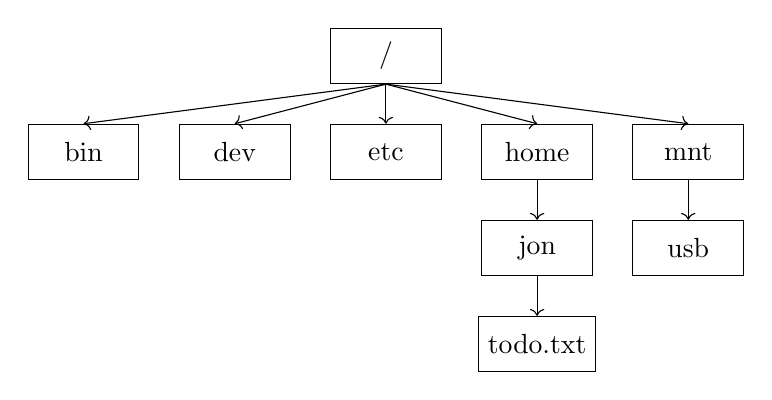
\begin{tikzpicture}[node distance=-2mm and 5mm]

        \node[draw,rectangle,minimum width=40,minimum height=20] (root)  {/};
        \node[draw,rectangle,minimum width=40,minimum height=20,yshift=-20] (etc) [below=of root] {etc};
        \node[draw,rectangle,minimum width=40,minimum height=20] (dev) [left=of etc] {dev};
        \node[draw,rectangle,minimum width=40,minimum height=20] (bin) [left=of dev] {bin};
        \node[draw,rectangle,minimum width=40,minimum height=20] (home) [right=of etc] {home};
        \node[draw,rectangle,minimum width=40,minimum height=20] (mnt) [right=of home] {mnt};
    
        \node[draw,rectangle,minimum width=40,minimum height=20,yshift=-20] (jon) [below=of home] {jon};
        \node[draw,rectangle,minimum width=40,minimum height=20,yshift=-20] (todotxt) [below=of jon] {todo.txt};
    
        \node[draw,rectangle,minimum width=40,minimum height=20,yshift=-20] (usb) [below=of mnt] {usb};
    
        \draw[->] (root.south) -- (bin.north);
        \draw[->] (root.south) -- (dev.north);
        \draw[->] (root.south) -- (etc.north);
        \draw[->] (root.south) -- (home.north);
        \draw[->] (root.south) -- (mnt.north);
        \draw[->] (home.south) -- (jon.north);
        \draw[->] (mnt.south) -- (usb.north);
        \draw[->] (jon.south) -- (todotxt.north);
    
      \end{tikzpicture}
    \end{center}

    Working Directory: /home/jon

    \leftspace{}What is the absolute and relative path to \textbf{todo.txt}?
    To \textbf{usb}?

  \end{slide}

  \begin{slide}
    
    \slidetitle{POSIX Filesystem}

    todo.txt Relative: ./todo.txt

    todo.txt Absolute: /home/jon/todo.txt

    usb Relative: ../../mnt/usb

    usb Absolute: /mnt/usb
    \medskip

    Special symbols:

    \leftspace{}. --- Current directory
    
    \leftspace{}.. ---  Parent directory

    \leftspace{}$\mathsf{\sim}$ --- User's home directory (\$HOME)

    Relative paths are calculated from current working directory (\$PWD)

  \end{slide}

  \begin{slide}
    
    \slidetitle{You Can Access Files Sequentially or Randomly}

    Sequential access

    \leftspace{}Each read advances the position inside the file

    \leftspace{}Writes are appended and the position set to the end afterwards
    \medskip

    Random access

    \leftspace{}Records can be read/written to the file in any order

    \leftspace{}A specific position is required for each operation

  \end{slide}

  \begin{slide}
    
    \slidetitle{POSIX Filesystem}

    \begin{minted}{c}
int open(const char *pathname, int flags, mode_t mode);

// flags can specify which operations: O_RDWR,O_WRONLY, O_RDWR
// also: O_APPEND moves the position to the end of the file initially

off_t lseek(int fd, off_t offset, int whence);

// lseek changes the position to the offset
// whence can be one of: SEEK_SET, SEEK_CUR, SEEK_END
//   set makes the offset absolute, cur and end are both relative
    \end{minted}
  \end{slide}

  \begin{slide}
    
    \slidetitle{Accessing Directory API}

    \begin{minted}{c}
DIR *opendir(char *path); // open directory
struct dirent *readdir(DIR *dir); // get next item
int closedir(DIR *dir); // close directory

void print_directory_contents(char *path) {
    DIR *dir = opendir(path);
    struct dirent *item;
    while (item = readdir(dir)) {
        printf("- %s\n", item->d_name);
    }
    closedir(path);
}
    \end{minted}

  \end{slide}

  \begin{slide}
    
    \slidetitle{File Tables Are Stored in the Process Control Block (PCB)}

    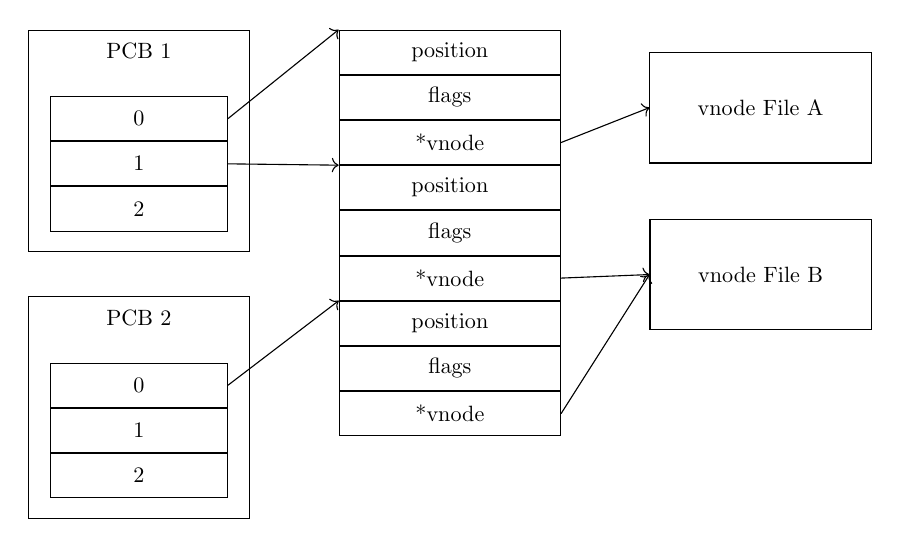
\begin{tikzpicture}[node distance=0mm and 0mm,scale=0.8, every node/.style={transform shape}]
      \node[rectangle,draw,minimum width=100,minimum height=100] (pcb1)      {};
      \node[rectangle,minimum width=100,minimum height=20,yshift=-20] (pcb11) [above=of pcb1] {PCB 1};
      \node[rectangle,draw,minimum width=80,minimum height=20,xshift=0,yshift=-10] (lof11) [below=of pcb11] {0};
      \node[rectangle,draw,minimum width=80,minimum height=20] (lof12) [below=of lof11] {1};
      \node[rectangle,draw,minimum width=80,minimum height=20] (lof13) [below=of lof12] {2};


      \node[rectangle,draw,minimum width=100,minimum height=100,yshift=-20] (pcb2)   [below=of pcb1]   {};
      \node[rectangle,minimum width=100,minimum height=20,yshift=-20] (pcb21) [above=of pcb2] {PCB 2};
      \node[rectangle,draw,minimum width=80,minimum height=20,xshift=0,yshift=-10] (lof21) [below=of pcb21] {0};
      \node[rectangle,draw,minimum width=80,minimum height=20] (lof22) [below=of lof21] {1};
      \node[rectangle,draw,minimum width=80,minimum height=20] (lof23) [below=of lof22] {2};

      \node[rectangle,draw,minimum width=100,minimum height=20,xshift=40,yshift=40] (gof1)   [right=of pcb1]   {position};
      \node[rectangle,draw,minimum width=100,minimum height=20] (gof2)   [below=of gof1]   {flags};
      \node[rectangle,draw,minimum width=100,minimum height=20] (gof3)   [below=of gof2]   {*vnode};

      \node[rectangle,draw,minimum width=100,minimum height=20] (gof4)   [below=of gof3]   {position};
      \node[rectangle,draw,minimum width=100,minimum height=20] (gof5)   [below=of gof4]   {flags};
      \node[rectangle,draw,minimum width=100,minimum height=20] (gof6)   [below=of gof5]   {*vnode};

      \node[rectangle,draw,minimum width=100,minimum height=20] (gof7)   [below=of gof6]   {position};
      \node[rectangle,draw,minimum width=100,minimum height=20] (gof8)   [below=of gof7]   {flags};
      \node[rectangle,draw,minimum width=100,minimum height=20] (gof9)   [below=of gof8]   {*vnode};

      \node[rectangle,draw,minimum width=100,minimum height=50,xshift=40,yshift=-25] (vnode1)  [right=of gof1]    {vnode File A};
      \node[rectangle,draw,minimum width=100,minimum height=50,yshift=-25] (vnode2)  [below=of vnode1]    {vnode File B};

      \draw[->] (lof11.east) -- (gof1.north west);
      \draw[->] (lof12.east) -- (gof4.north west);
      \draw[->] (lof21.east) -- (gof7.north west);

      \draw[->] (gof3.east) -- (vnode1.west);
      \draw[->] (gof6.east) -- (vnode2.west);
      \draw[->] (gof9.east) -- (vnode2.west);        
    \end{tikzpicture}
  \end{slide}

  \begin{slide}
    
    \slidetitle{Each Process Contains a File Table in its PCB}

    A File Descriptor is an index in the table
    \medskip

    Each item points to a system-wide \textit{global open file table}
    \medskip

    The GOF table holds information about the seek position and flags

    \leftspace{}It also points to a \textit{VNode} (supports read/write/etc)
    \medskip

    A vnode (virtual mode) holds information about the file

    \leftspace{}vnodes can represent regular files, pipes, network sockets, etc.

  \end{slide}

  \begin{slide}
    
    \slidetitle{Remember What Happens In A Fork}

    PCB is copied on fork
    \medskip

    Specifically for us, the local open file table gets inherited
    \medskip

    Both PCBs point to the same Global Open File Table entry
  \end{slide}

  \begin{slide}
    
    \slidetitle{Both Processes Point to the Same GOF Entry}

    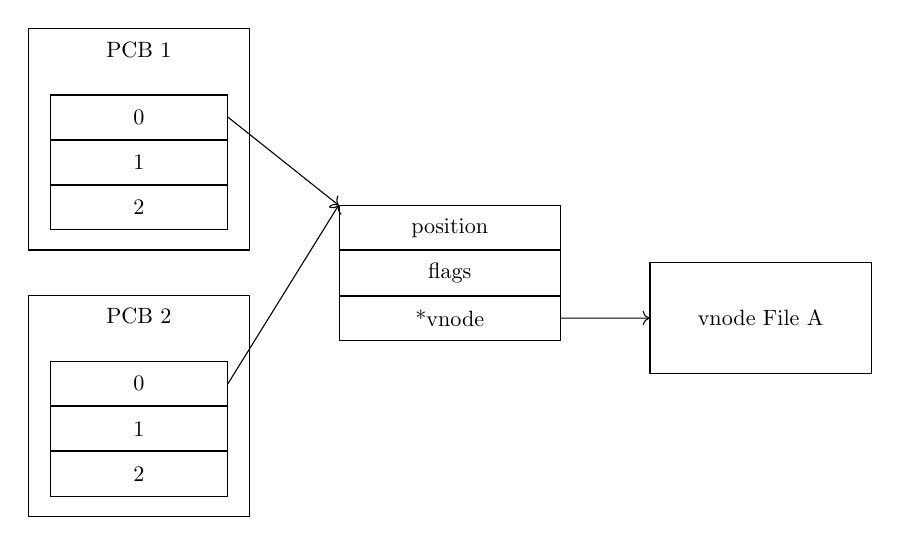
\begin{tikzpicture}[node distance=0mm and 0mm,scale=0.8, every node/.style={transform shape}]
      
      \node[rectangle,draw,minimum width=100,minimum height=100] (pcb1)      {};
      \node[rectangle,minimum width=100,minimum height=20,yshift=-20] (pcb11) [above=of pcb1] {PCB 1};
      \node[rectangle,draw,minimum width=80,minimum height=20,xshift=0,yshift=-10] (lof11) [below=of pcb11] {0};
      \node[rectangle,draw,minimum width=80,minimum height=20] (lof12) [below=of lof11] {1};
      \node[rectangle,draw,minimum width=80,minimum height=20] (lof13) [below=of lof12] {2};


      \node[rectangle,draw,minimum width=100,minimum height=100,yshift=-20] (pcb2)   [below=of pcb1]   {};
      \node[rectangle,minimum width=100,minimum height=20,yshift=-20] (pcb21) [above=of pcb2] {PCB 2};
      \node[rectangle,draw,minimum width=80,minimum height=20,xshift=0,yshift=-10] (lof21) [below=of pcb21] {0};
      \node[rectangle,draw,minimum width=80,minimum height=20] (lof22) [below=of lof21] {1};
      \node[rectangle,draw,minimum width=80,minimum height=20] (lof23) [below=of lof22] {2};

      \node[rectangle,draw,minimum width=100,minimum height=20,xshift=40,yshift=-40] (gof1)   [right=of pcb1]   {position};
      \node[rectangle,draw,minimum width=100,minimum height=20] (gof2)   [below=of gof1]   {flags};
      \node[rectangle,draw,minimum width=100,minimum height=20] (gof3)   [below=of gof2]   {*vnode};

      \node[rectangle,draw,minimum width=100,minimum height=50,xshift=40] (vnode1)  [right=of gof3]    {vnode File A};

      \draw[->] (lof11.east) -- (gof1.north west);
      \draw[->] (lof21.east) -- (gof1.north west);

      \draw[->] (gof3.east) -- (vnode1.west);    

    \end{tikzpicture}

  \end{slide}

  \begin{slide}
    
    \slidetitle{There Are Some ``Gotchas'' For This Sharing}

    Current position in file is shared between both processes
    \medskip

    Seek in one process leads to seek in all other processes using the same GOF
    entry
    \medskip

    Opening the same file in both processes after forking creates multiple
    GOF entries

  \end{slide}

  \begin{slide}
    
    \slidetitle{How many LOF and GOF Entries Exist? What is the Relationship?}

    \begin{minted}{c}
open("todo.txt", O_RDONLY);
fork();
open("b.txt", O_RDONLY);
    \end{minted}
    \medskip

    Assume there are no previously opened files (not even the standard ones)

  \end{slide}

  \begin{slide}
    
    \slidetitle{There are 2 LOF Entries Each, and 3 GOF Entries}

    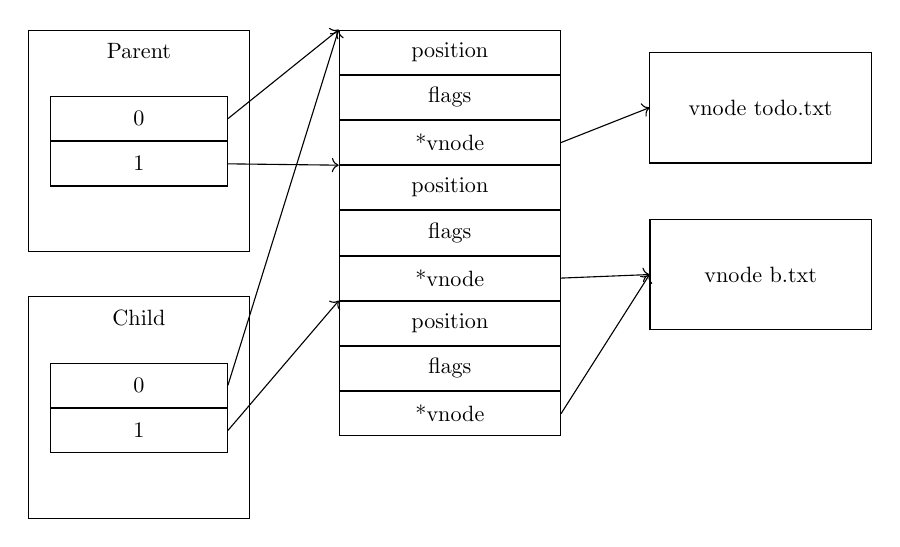
\begin{tikzpicture}[node distance=0mm and 0mm,scale=0.8, every node/.style={transform shape}]
        
      \node[rectangle,draw,minimum width=100,minimum height=100] (pcb1)      {};
      \node[rectangle,minimum width=100,minimum height=20,yshift=-20] (pcb11) [above=of pcb1] {Parent};
      \node[rectangle,draw,minimum width=80,minimum height=20,xshift=0,yshift=-10] (lof11) [below=of pcb11] {0};
      \node[rectangle,draw,minimum width=80,minimum height=20] (lof12) [below=of lof11] {1};


      \node[rectangle,draw,minimum width=100,minimum height=100,yshift=-20] (pcb2)   [below=of pcb1]   {};
      \node[rectangle,minimum width=100,minimum height=20,yshift=-20] (pcb21) [above=of pcb2] {Child};
      \node[rectangle,draw,minimum width=80,minimum height=20,xshift=0,yshift=-10] (lof21) [below=of pcb21] {0};
      \node[rectangle,draw,minimum width=80,minimum height=20] (lof22) [below=of lof21] {1};

      \node[rectangle,draw,minimum width=100,minimum height=20,xshift=40,yshift=40] (gof1)   [right=of pcb1]   {position};
      \node[rectangle,draw,minimum width=100,minimum height=20] (gof2)   [below=of gof1]   {flags};
      \node[rectangle,draw,minimum width=100,minimum height=20] (gof3)   [below=of gof2]   {*vnode};

      \node[rectangle,draw,minimum width=100,minimum height=20] (gof4)   [below=of gof3]   {position};
      \node[rectangle,draw,minimum width=100,minimum height=20] (gof5)   [below=of gof4]   {flags};
      \node[rectangle,draw,minimum width=100,minimum height=20] (gof6)   [below=of gof5]   {*vnode};

      \node[rectangle,draw,minimum width=100,minimum height=20] (gof7)   [below=of gof6]   {position};
      \node[rectangle,draw,minimum width=100,minimum height=20] (gof8)   [below=of gof7]   {flags};
      \node[rectangle,draw,minimum width=100,minimum height=20] (gof9)   [below=of gof8]   {*vnode};

      \node[rectangle,draw,minimum width=100,minimum height=50,xshift=40,yshift=-25] (vnode1)  [right=of gof1]    {vnode todo.txt};
      \node[rectangle,draw,minimum width=100,minimum height=50,yshift=-25] (vnode2)  [below=of vnode1]    {vnode b.txt};

      \draw[->] (lof11.east) -- (gof1.north west);
      \draw[->] (lof12.east) -- (gof4.north west);
      \draw[->] (lof21.east) -- (gof1.north west);
      \draw[->] (lof22.east) -- (gof7.north west);

      \draw[->] (gof3.east) -- (vnode1.west);
      \draw[->] (gof6.east) -- (vnode2.west);
      \draw[->] (gof9.east) -- (vnode2.west);        

    \end{tikzpicture}
  \end{slide}

  \begin{slide}
    
    \slidetitle{How Do We Store Files? Contiguous Allocation?}
    
    \begin{center}
        
      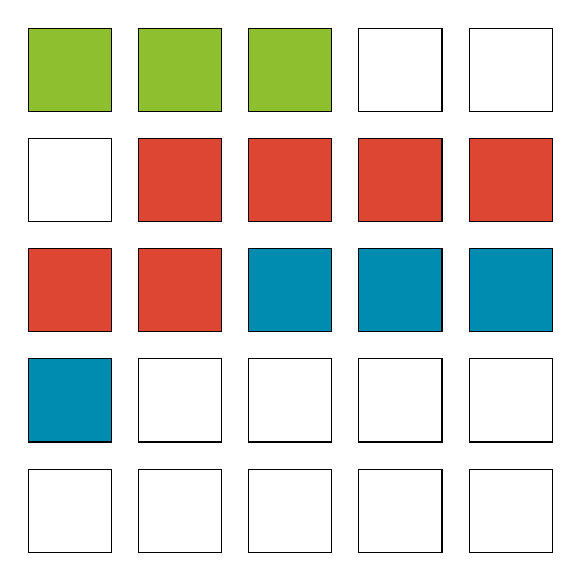
\begin{tikzpicture}[node distance=14mm and 14mm]

        \node[rectangle,draw,minimum width=30,minimum height=30,fill=pantone376] (b1)   {};
        \node[rectangle,draw,minimum width=30,minimum height=30,fill=pantone376] (b2) [right of=b1]  {};
        \node[rectangle,draw,minimum width=30,minimum height=30,fill=pantone376] (b3) [right of=b2]  {};
        \node[rectangle,draw,minimum width=30,minimum height=30] (b4) [right of=b3]  {};
        \node[rectangle,draw,minimum width=30,minimum height=30] (b5) [right of=b4]  {};

        \node[rectangle,draw,minimum width=30,minimum height=30] (b6) [below of=b1]  {};
        \node[rectangle,draw,minimum width=30,minimum height=30,fill=pantonewarmred] (b7) [right of=b6]  {};
        \node[rectangle,draw,minimum width=30,minimum height=30,fill=pantonewarmred] (b8) [right of=b7]  {};
        \node[rectangle,draw,minimum width=30,minimum height=30,fill=pantonewarmred] (b9) [right of=b8]  {};
        \node[rectangle,draw,minimum width=30,minimum height=30,fill=pantonewarmred] (b10) [right of=b9]  {};

        \node[rectangle,draw,minimum width=30,minimum height=30,fill=pantonewarmred] (b11) [below of=b6]  {};
        \node[rectangle,draw,minimum width=30,minimum height=30,fill=pantonewarmred] (b12) [right of=b11]  {};
        \node[rectangle,draw,minimum width=30,minimum height=30,fill=pantone633] (b13) [right of=b12]  {};
        \node[rectangle,draw,minimum width=30,minimum height=30,fill=pantone633] (b14) [right of=b13]  {};
        \node[rectangle,draw,minimum width=30,minimum height=30,fill=pantone633] (b15) [right of=b14]  {};

        \node[rectangle,draw,minimum width=30,minimum height=30,fill=pantone633] (b16) [below of=b11]  {};
        \node[rectangle,draw,minimum width=30,minimum height=30] (b17) [right of=b16]  {};
        \node[rectangle,draw,minimum width=30,minimum height=30] (b18) [right of=b17]  {};
        \node[rectangle,draw,minimum width=30,minimum height=30] (b19) [right of=b18]  {};
        \node[rectangle,draw,minimum width=30,minimum height=30] (b20) [right of=b19]  {};

        \node[rectangle,draw,minimum width=30,minimum height=30] (b21) [below of=b16]  {};
        \node[rectangle,draw,minimum width=30,minimum height=30] (b22) [right of=b21]  {};
        \node[rectangle,draw,minimum width=30,minimum height=30] (b23) [right of=b22]  {};
        \node[rectangle,draw,minimum width=30,minimum height=30] (b24) [right of=b23]  {};
        \node[rectangle,draw,minimum width=30,minimum height=30] (b25) [right of=b24]  {};

      \end{tikzpicture}

    \end{center}
  \end{slide}

  \begin{slide}
    
    \slidetitle{Contiguous Allocation Is Fast, If There Are No Modifications}

    Space efficient: Only start block and \# of blocks need to be stored
    \medskip

    Fast random access: $block = floor(\frac{offset}{blocksize})$
    \medskip

    Files can not grow easily

    \leftspace{}Internal fragmentation (may not fill a block)
    
    \leftspace{}External fragmentation when files are deleted or truncated
  \end{slide}

  \begin{slide}
    
    \slidetitle{
      What About Storing Like a Free List of Pages?
    
      Linked Allocation
    }

    \begin{center}
      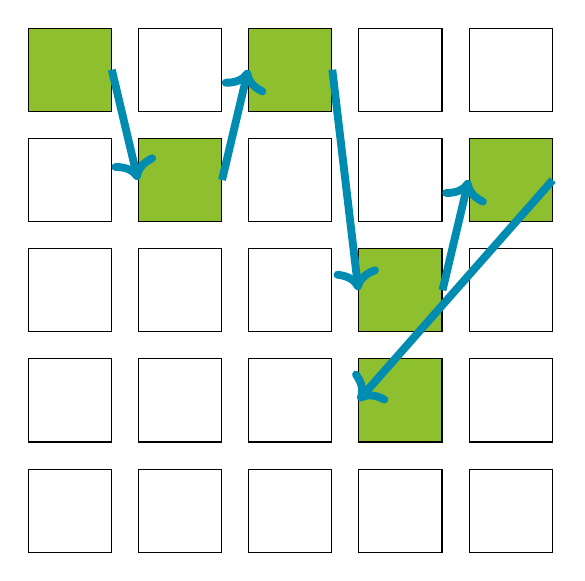
\begin{tikzpicture}[node distance=14mm and 14mm]

        \node[rectangle,draw,minimum width=30,minimum height=30,fill=pantone376] (b1)   {};
        \node[rectangle,draw,minimum width=30,minimum height=30] (b2) [right of=b1]  {};
        \node[rectangle,draw,minimum width=30,minimum height=30,fill=pantone376] (b3) [right of=b2]  {};
        \node[rectangle,draw,minimum width=30,minimum height=30] (b4) [right of=b3]  {};
        \node[rectangle,draw,minimum width=30,minimum height=30] (b5) [right of=b4]  {};

        \node[rectangle,draw,minimum width=30,minimum height=30] (b6) [below of=b1]  {};
        \node[rectangle,draw,minimum width=30,minimum height=30,fill=pantone376] (b7) [right of=b6]  {};
        \node[rectangle,draw,minimum width=30,minimum height=30] (b8) [right of=b7]  {};
        \node[rectangle,draw,minimum width=30,minimum height=30] (b9) [right of=b8]  {};
        \node[rectangle,draw,minimum width=30,minimum height=30,fill=pantone376] (b10) [right of=b9]  {};

        \node[rectangle,draw,minimum width=30,minimum height=30] (b11) [below of=b6]  {};
        \node[rectangle,draw,minimum width=30,minimum height=30] (b12) [right of=b11]  {};
        \node[rectangle,draw,minimum width=30,minimum height=30] (b13) [right of=b12]  {};
        \node[rectangle,draw,minimum width=30,minimum height=30,fill=pantone376] (b14) [right of=b13]  {};
        \node[rectangle,draw,minimum width=30,minimum height=30] (b15) [right of=b14]  {};

        \node[rectangle,draw,minimum width=30,minimum height=30] (b16) [below of=b11]  {};
        \node[rectangle,draw,minimum width=30,minimum height=30] (b17) [right of=b16]  {};
        \node[rectangle,draw,minimum width=30,minimum height=30] (b18) [right of=b17]  {};
        \node[rectangle,draw,minimum width=30,minimum height=30,fill=pantone376] (b19) [right of=b18]  {};
        \node[rectangle,draw,minimum width=30,minimum height=30] (b20) [right of=b19]  {};

        \node[rectangle,draw,minimum width=30,minimum height=30] (b21) [below of=b16]  {};
        \node[rectangle,draw,minimum width=30,minimum height=30] (b22) [right of=b21]  {};
        \node[rectangle,draw,minimum width=30,minimum height=30] (b23) [right of=b22]  {};
        \node[rectangle,draw,minimum width=30,minimum height=30] (b24) [right of=b23]  {};
        \node[rectangle,draw,minimum width=30,minimum height=30] (b25) [right of=b24]  {};

        \draw[->,line width=1mm,draw=pantone633] (b1.east) -- (b7.west);
        \draw[->,line width=1mm,draw=pantone633] (b7.east) -- (b3.west);
        \draw[->,line width=1mm,draw=pantone633] (b3.east) -- (b14.west);
        \draw[->,line width=1mm,draw=pantone633] (b14.east) -- (b10.west);
        \draw[->,line width=1mm,draw=pantone633] (b10.east) -- (b19.west);

      \end{tikzpicture}
    \end{center}
  \end{slide}

  \begin{slide}
    
    \slidetitle{Linked Allocation Has Slow Random Access}
    
    Space efficient: Only start block needs to be stored

    \leftspace{}Blocks need to store a pointer to the next block (block is slightly smaller)
    \medskip

    Files can grow/shrink

    \leftspace{}No external fragmentation

    \leftspace{}Internal fragmentation
    \medskip

    How can we increase random access speed? We need to walk each block

    \leftspace{}Each block may be located far away (it will never be cached)

  \end{slide}

  \begin{slide}

    \slidetitle{File Allocation Table Moves The List to a Separate Table}
    
    \begin{center}
        
      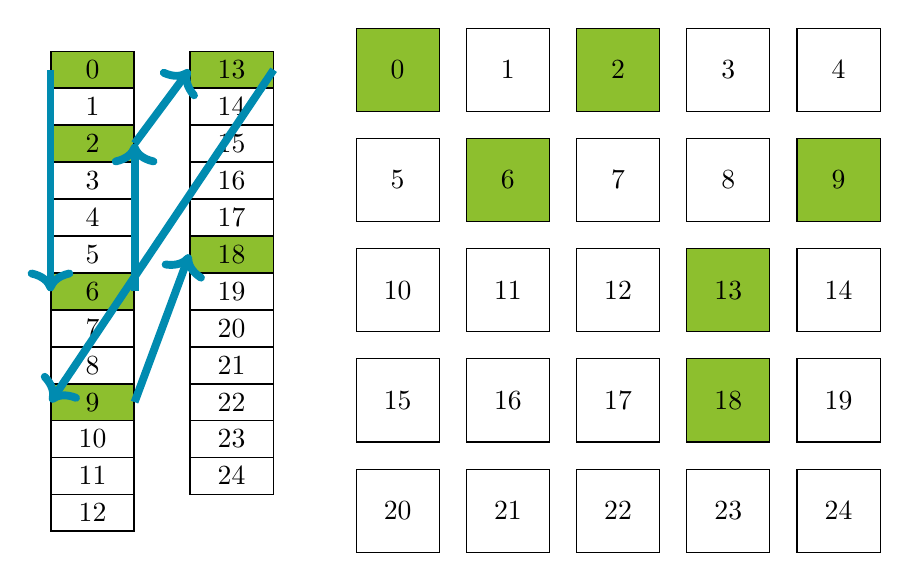
\begin{tikzpicture}[node distance=14mm and 14mm]

        \node[rectangle,draw,minimum width=30,minimum height=30,fill=pantone376] (b1)   {0};
        \node[rectangle,draw,minimum width=30,minimum height=30] (b2) [right of=b1]  {1};
        \node[rectangle,draw,minimum width=30,minimum height=30,fill=pantone376] (b3) [right of=b2]  {2};
        \node[rectangle,draw,minimum width=30,minimum height=30] (b4) [right of=b3]  {3};
        \node[rectangle,draw,minimum width=30,minimum height=30] (b5) [right of=b4]  {4};

        \node[rectangle,draw,minimum width=30,minimum height=30] (b6) [below of=b1]  {5};
        \node[rectangle,draw,minimum width=30,minimum height=30,fill=pantone376] (b7) [right of=b6]  {6};
        \node[rectangle,draw,minimum width=30,minimum height=30] (b8) [right of=b7]  {7};
        \node[rectangle,draw,minimum width=30,minimum height=30] (b9) [right of=b8]  {8};
        \node[rectangle,draw,minimum width=30,minimum height=30,fill=pantone376] (b10) [right of=b9]  {9};

        \node[rectangle,draw,minimum width=30,minimum height=30] (b11) [below of=b6]  {10};
        \node[rectangle,draw,minimum width=30,minimum height=30] (b12) [right of=b11]  {11};
        \node[rectangle,draw,minimum width=30,minimum height=30] (b13) [right of=b12]  {12};
        \node[rectangle,draw,minimum width=30,minimum height=30,fill=pantone376] (b14) [right of=b13]  {13};
        \node[rectangle,draw,minimum width=30,minimum height=30] (b15) [right of=b14]  {14};

        \node[rectangle,draw,minimum width=30,minimum height=30] (b16) [below of=b11]  {15};
        \node[rectangle,draw,minimum width=30,minimum height=30] (b17) [right of=b16]  {16};
        \node[rectangle,draw,minimum width=30,minimum height=30] (b18) [right of=b17]  {17};
        \node[rectangle,draw,minimum width=30,minimum height=30,fill=pantone376] (b19) [right of=b18]  {18};
        \node[rectangle,draw,minimum width=30,minimum height=30] (b20) [right of=b19]  {19};

        \node[rectangle,draw,minimum width=30,minimum height=30] (b21) [below of=b16]  {20};
        \node[rectangle,draw,minimum width=30,minimum height=30] (b22) [right of=b21]  {21};
        \node[rectangle,draw,minimum width=30,minimum height=30] (b23) [right of=b22]  {22};
        \node[rectangle,draw,minimum width=30,minimum height=30] (b24) [right of=b23]  {23};
        \node[rectangle,draw,minimum width=30,minimum height=30] (b25) [right of=b24]  {24};

        \node[rectangle,draw,minimum width=30,minimum height=10,xshift=-40,fill=pantone376] (fat1) [left=of b1] {0};
        \node[rectangle,draw,minimum width=30,minimum height=10,yshift=40] (fat2) [below=of fat1] {1};
        \node[rectangle,draw,minimum width=30,minimum height=10,yshift=40,fill=pantone376] (fat3) [below=of fat2] {2};
        \node[rectangle,draw,minimum width=30,minimum height=10,yshift=40] (fat4) [below=of fat3] {3};
        \node[rectangle,draw,minimum width=30,minimum height=10,yshift=40] (fat5) [below=of fat4] {4};
        \node[rectangle,draw,minimum width=30,minimum height=10,yshift=40] (fat6) [below=of fat5] {5};
        \node[rectangle,draw,minimum width=30,minimum height=10,yshift=40,fill=pantone376] (fat7) [below=of fat6] {6};
        \node[rectangle,draw,minimum width=30,minimum height=10,yshift=40] (fat8) [below=of fat7] {7};
        \node[rectangle,draw,minimum width=30,minimum height=10,yshift=40] (fat9) [below=of fat8] {8};
        \node[rectangle,draw,minimum width=30,minimum height=10,yshift=40,fill=pantone376] (fat10) [below=of fat9] {9};
        \node[rectangle,draw,minimum width=30,minimum height=10,yshift=40] (fat11) [below=of fat10] {10};
        \node[rectangle,draw,minimum width=30,minimum height=10,yshift=40] (fat12) [below=of fat11] {11};
        \node[rectangle,draw,minimum width=30,minimum height=10,yshift=40] (fat13) [below=of fat12] {12};

        \node[rectangle,draw,minimum width=30,minimum height=10,xshift=-20,fill=pantone376] (fat14) [right=of fat1] {13};
        \node[rectangle,draw,minimum width=30,minimum height=10,yshift=40] (fat15) [below=of fat14] {14};

        \node[rectangle,draw,minimum width=30,minimum height=10,yshift=40] (fat16) [below=of fat15] {15};
        \node[rectangle,draw,minimum width=30,minimum height=10,yshift=40] (fat17) [below=of fat16] {16};
        \node[rectangle,draw,minimum width=30,minimum height=10,yshift=40] (fat18) [below=of fat17] {17};
        \node[rectangle,draw,minimum width=30,minimum height=10,yshift=40,fill=pantone376] (fat19) [below=of fat18] {18};
        \node[rectangle,draw,minimum width=30,minimum height=10,yshift=40] (fat20) [below=of fat19] {19};
        \node[rectangle,draw,minimum width=30,minimum height=10,yshift=40] (fat21) [below=of fat20] {20};
        \node[rectangle,draw,minimum width=30,minimum height=10,yshift=40] (fat22) [below=of fat21] {21};
        \node[rectangle,draw,minimum width=30,minimum height=10,yshift=40] (fat23) [below=of fat22] {22};
        \node[rectangle,draw,minimum width=30,minimum height=10,yshift=40] (fat24) [below=of fat23] {23};
        \node[rectangle,draw,minimum width=30,minimum height=10,yshift=40] (fat25) [below=of fat24] {24};

        \draw[->,line width=1mm,color=pantone633] (fat1.west) -- (fat7.west);
        \draw[->,line width=1mm,color=pantone633] (fat7.east) -- (fat3.east);
        \draw[->,line width=1mm,color=pantone633] (fat3.east) -- (fat14.west);
        \draw[->,line width=1mm,color=pantone633] (fat14.east) -- (fat10.west);
        \draw[->,line width=1mm,color=pantone633] (fat10.east) -- (fat19.west);

      \end{tikzpicture}

    \end{center}

  \end{slide}

  \begin{slide}
    
    \slidetitle{File Allocation Table (FAT) is Similar to Linked Allocation}

    Files can grow/shrink

    \leftspace{}No external fragmentation

    \leftspace{}Internal fragmentation
    \medskip

    \vspace{2em}

    Fast random access: FAT can be held in memory/cache
    
    \leftspace{}FAT size is linear to disk size: can become very large
    \medskip

    How can we further increase random access speed?

  \end{slide}

  \begin{slide}
    
    \slidetitle{Indexed Allocation Maps Each Block Directly}

    \begin{center}
      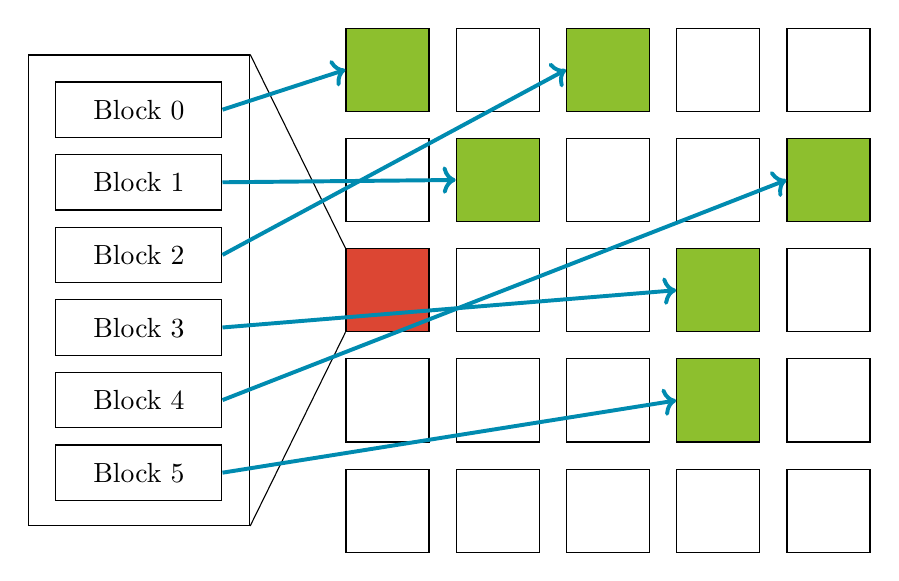
\begin{tikzpicture}[node distance=14mm and 14mm]

        \node[rectangle,draw,minimum width=30,minimum height=30,fill=pantone376] (b1)   {};
        \node[rectangle,draw,minimum width=30,minimum height=30] (b2) [right of=b1]  {};
        \node[rectangle,draw,minimum width=30,minimum height=30,fill=pantone376] (b3) [right of=b2]  {};
        \node[rectangle,draw,minimum width=30,minimum height=30] (b4) [right of=b3]  {};
        \node[rectangle,draw,minimum width=30,minimum height=30] (b5) [right of=b4]  {};

        \node[rectangle,draw,minimum width=30,minimum height=30] (b6) [below of=b1]  {};
        \node[rectangle,draw,minimum width=30,minimum height=30,fill=pantone376] (b7) [right of=b6]  {};
        \node[rectangle,draw,minimum width=30,minimum height=30] (b8) [right of=b7]  {};
        \node[rectangle,draw,minimum width=30,minimum height=30] (b9) [right of=b8]  {};
        \node[rectangle,draw,minimum width=30,minimum height=30,fill=pantone376] (b10) [right of=b9]  {};

        \node[rectangle,draw,minimum width=30,minimum height=30,fill=pantonewarmred] (b11) [below of=b6]  {};
        \node[rectangle,draw,minimum width=30,minimum height=30] (b12) [right of=b11]  {};
        \node[rectangle,draw,minimum width=30,minimum height=30] (b13) [right of=b12]  {};
        \node[rectangle,draw,minimum width=30,minimum height=30,fill=pantone376] (b14) [right of=b13]  {};
        \node[rectangle,draw,minimum width=30,minimum height=30] (b15) [right of=b14]  {};

        \node[rectangle,draw,minimum width=30,minimum height=30] (b16) [below of=b11]  {};
        \node[rectangle,draw,minimum width=30,minimum height=30] (b17) [right of=b16]  {};
        \node[rectangle,draw,minimum width=30,minimum height=30] (b18) [right of=b17]  {};
        \node[rectangle,draw,minimum width=30,minimum height=30,fill=pantone376] (b19) [right of=b18]  {};
        \node[rectangle,draw,minimum width=30,minimum height=30] (b20) [right of=b19]  {};

        \node[rectangle,draw,minimum width=30,minimum height=30] (b21) [below of=b16]  {};
        \node[rectangle,draw,minimum width=30,minimum height=30] (b22) [right of=b21]  {};
        \node[rectangle,draw,minimum width=30,minimum height=30] (b23) [right of=b22]  {};
        \node[rectangle,draw,minimum width=30,minimum height=30] (b24) [right of=b23]  {};
        \node[rectangle,draw,minimum width=30,minimum height=30] (b25) [right of=b24]  {};

        \node[rectangle,draw,minimum width=80,minimum height=170,xshift=-50] (index) [left of=b11]  {};
        \node[rectangle,draw,minimum width=60,minimum height=20,yshift=-70] (index1) [above=of index] {Block 0};
        \node[rectangle,draw,minimum width=60,minimum height=20,yshift=34] (index2) [below=of index1] {Block 1};
        \node[rectangle,draw,minimum width=60,minimum height=20,yshift=34] (index3) [below=of index2] {Block 2};
        \node[rectangle,draw,minimum width=60,minimum height=20,yshift=34] (index4) [below=of index3] {Block 3};
        \node[rectangle,draw,minimum width=60,minimum height=20,yshift=34] (index5) [below=of index4] {Block 4};
        \node[rectangle,draw,minimum width=60,minimum height=20,yshift=34] (index6) [below=of index5] {Block 5};

        \draw[-] (index.north east) -- (b11.north west);
        \draw[-] (index.south east) -- (b11.south west);

        \draw[->,line width=0.5mm,color=pantone633] (index1.east) -- (b1.west);
        \draw[->,line width=0.5mm,color=pantone633] (index2.east) -- (b7.west);
        \draw[->,line width=0.5mm,color=pantone633] (index3.east) -- (b3.west);
        \draw[->,line width=0.5mm,color=pantone633] (index4.east) -- (b14.west);
        \draw[->,line width=0.5mm,color=pantone633] (index5.east) -- (b10.west);
        \draw[->,line width=0.5mm,color=pantone633] (index6.east) -- (b19.west);

      \end{tikzpicture}
    \end{center}

  \end{slide}

  \begin{slide}
    
    \slidetitle{For Indexed Allocation, Each File Needs an Index Block}

    Files can still grow/shrink

    \leftspace{}No external fragmentation

    \leftspace{}Internal fragmentation
    \medskip

    Fast random access
    \medskip

    File size limited by the maximum size of the index block (fit it in one block)

  \end{slide}

  \begin{slide}
    
    \slidetitle{Indexed Allocation Problem}
    
    Assume this scenario:
    \begin{itemize}
      \item An index block stores pointers to data blocks only (no meta information)
      \item A disk block is 8~KiB in size
      \item A pointer to a block is 4~Bytes
    \end{itemize}
    \medskip

    What is the maximum size of a file managed by this index block?

  \end{slide}

  \begin{slide}
    
    \slidetitle{Indexed Allocation Solution}
    
    Assume this scenario:
    \begin{itemize}
      \item An index block stores pointers to data blocks only (no meta information)
      \item A disk block is 8~KiB in size
      \item A pointer to a block is 4~Bytes
    \end{itemize}
    \medskip

    \# of pointers = $\mathsf{\frac{8 KiB}{4 B} \frac{2^{13} B}{2^2 B} = 2^{11}}$

    \# of addressable blocks = \# of pointers

    Total of bytes = $\mathsf{2^{11} \times 2^{13} = 2^{24} = 16 MiB}$

  \end{slide}

  \begin{slide}
    
    \slidetitle{Filesystems Enable Persistence}

    They describe how files are stored on disks:
    \begin{itemize}
      \item API-wise you can open files, and change the position to read/write
            at
      \item Each process has a local open file and there's a global open file
            table
      \item There's multiple allocation strategies: contiguous, linked, FAT, indexed
    \end{itemize}

  \end{slide}

\end{document}
